\expandafter\ifx\csname ifdraft\endcsname\relax
 \begin{document}
\fi

\section{製作}

\subsection{全体構成}

装置全体の構成図を以下に示す.

\subsection{マスク}

\subsubsection{呼気収集マスク}

呼気収集マスクには,仰木研究室内で以前に製作されたマスクを使用した.このマスクは,アクリル板を組み合わせて顔に合うような形状を構成し,吸気及び呼気用の通気口を設けた物である.顔に当たる部分にはウレタンフォーム製のクッションを取り付け,頭に取り付けられるように市販のガスマスクから流用したバンドが取り付けてある.

\subsubsection{逆止弁}

呼気を正確に収集するために,呼吸代謝測定装置のマスクの吸気・呼気部分には逆流防止弁を取り付ける必要がある.今回使用した逆止弁は,運動時に使用するマスクに取り付けるために安価に販売されているものである.薄いシリコーンゴム製の膜が1方向のみに膨らむことで気体の逆流を防止する.マスク本体には3Dプリンターで製作したスペーサーで径を合わせた上でネジで取り付けている.

\subsection{換気量V_Eの計測}

\subsubsection{計測方式}

換気量V_Eを計測するための流量計には,マイコン工作用として市販されている水流計を使用した.

気体の流量を計測するための流量計の原理としては,差圧流量計と超音波流量計,タービン流量計などがある.差圧流量計は流路内に絞り機構を設け,その前後に発生する圧力差を測ることで流量を計測する方式である.超音波流量計は,流路内を流れる流体に超音波を照射することで流量を計測する方式である.タービン流量計は,流路にタービンを設置し,流体によって回転するタービンの回転数によって流量を計測する方式である.タービン流量計は単純な構造であり,他の方式に比べて微細ではない構造なので,水流計として安価に市販されている.呼吸代謝測定装置のうち,流量計は高価な部品であり,全体の価格を抑えるためにタービン流量計を使用した.

今回使用した流量計はYF-S201という名称で販売されているもので,流路に対してタービンの軸が垂直に取り付けられている接線流羽根車式のタービン流量計である.タービンの回転数に応じてホール素子が矩形波の信号を出力する.主な仕様を表\ref{tb:YFS201_specsheet}に示す.

\begin{table}[h]
  \begin{center}
  \caption{YF-S201 主な公称仕様}
  \label{tb:YFS201_specsheet}
    \begin{tabular}{lc}
      流路外径 & 20mm \\
      入口内径 & 9mm \\
      出口内径 & 12mm \\
      動作流量 & 1-30L/min \\
      関係式 & 1L_{水} = 450pulse
    \end{tabular}
  \end{center}
\end{table}

\subsubsection{タービン式水流計の流量関係式の算出}

仕様によれば,YF-S201は水流1Lあたりに450個の矩形波を出力する.これは水流が流れる時の値なので,空気の流量計として使用するためには空気が流れる際の関係式を求める必要がある.今回はこれを実験で求めた.

\begin{figure}[h]
  \begin{center}
    \label{fig:flowsensor_calibrate}
    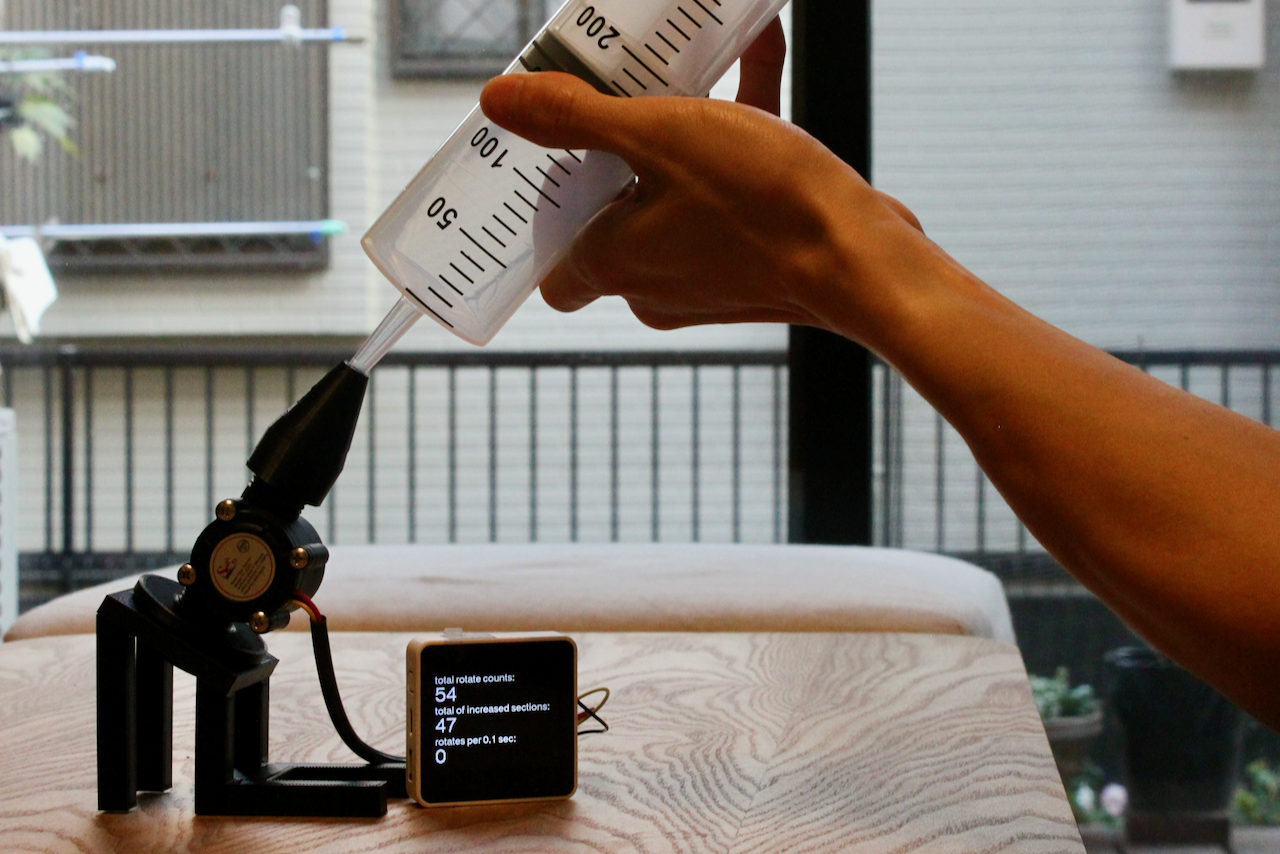
\includegraphics[width=8cm]{fig/flowsensor_calibrate.png}
    \caption{流量関係式算出用の実験}
  \end{center}
\end{figure}

図\ref{fig:flowsensor_calibrate}は実験の全景である.
空気の量を正確に測りとれるシリンジを流量計の入り口に接続し,一定量の空気を送り込んだ時のタービンの回転数,すなわち矩形波の数を計測した.
送り込む空気の量は,入手が可能であったシリンジの最大サイズから300mLとした.シリンジのピストンを押す速さが出来る限り一定になるように注意しながら手でピストンを押した.シリンジと流量計の接続部は空気が漏れないようにするためにジョイント部品を製作した.シリンジのノズルと流量計のネジ部分を接続する部品を3Dプリンターで製作した.また,予備実験において,シリンジのノズルから出た高圧の空気が流量計のタービンの羽根に直撃すると回転数が多くなることが確認できたため,図\ref{fig:syringe_cone}のように,ノズルから出た空気が一度中央に当たってから流量計へと流れる形状とした.

\begin{figure}[h]
  \begin{center}
    \label{fig:syringe_cone}
    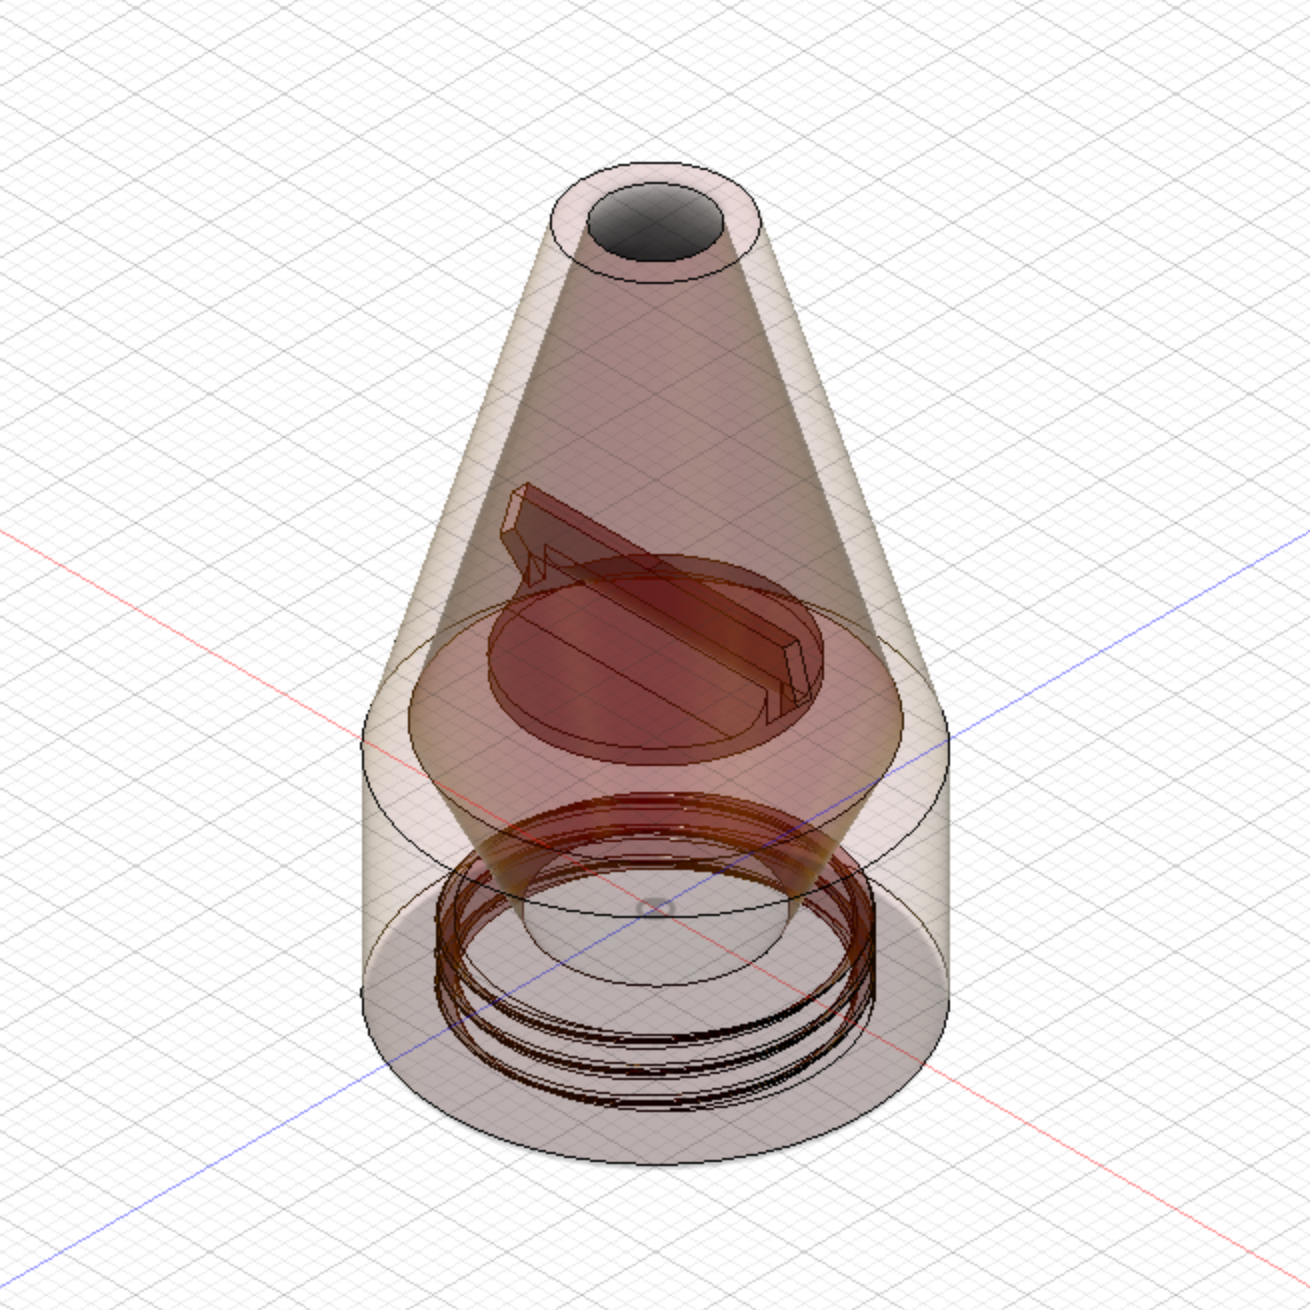
\includegraphics[width=8cm]{fig/syringe_cone}
    \caption{シリンジと流量計の接続用ジョイント部品}
  \end{center}
\end{figure}

今回使用した流量計はタービン軸の回転の滑らかさが重力に影響されやすいことが予備実験から分かった.そこで,流量計の角度を実際にマスクに取り付けた際の顔を正面に向けた場合を想定し,60度に保持するための治具を3Dプリンターで製作した.
今回の装置では流量計は呼気側の逆止弁の排気側に取り付けられるため,呼気から吸気に切り替わった後も一定時間タービン流量計が空転する.正しく換気量を計測するためにはこの空転分の回転数を除外する必要がある.そこで,回転数を計測するプログラムにこれを除外する処理を加えた.0.1秒毎の回転数を計測し,一個前の区間と比べて値が減少している区間の回転数を除外するという方法で行った.
以上の処理を行い,空転分を除外した回転数を計測するプログラムをM5Stack Core2で動作させ,200回分のデータの代表値を0.3mLの空気が流れた時の回転数とするという方法で流量関係式の算出を行った.結果は以下の通りである.

ミキシングチャンバー方式で換気量を測定するため,マスクの呼気方向にのみ解放される弁の先に取り付けた流量計で換気量を測定する

今回はマイコンなどに接続する水量計として安価に市販されているタービン流量計を流量計に用いた.YF-S201という名称で販売されているもので,タービンの回転数をホール素子センサーによって測定するものである.

呼気のような微小な気体の流量を測定するための流量計には,差圧流量計,超音波流量計,タービン流量計などが用いられる.

差圧流量計は,流路内に絞り機構を設置し,その前後に設置した圧力計から得られる圧力差から流量を測定する方式である.絞り機構としてオリフィスプレートを用いたものはオリフィス流量計と呼ばれる.
超音波流量計は流路内を流れる流体に超音波を照射することで流量を測定する方式である.
タービン流量計は流路にタービンを設置し,流体によって回転するタービンの回転数によって流量を測定する方式である.

%差圧流量計は,流路内に絞り機構を設置し,その前後に設置した圧力計から得られる圧力差から流量を測定する方式である.絞り機構としてオリフィスプレートを用いたもの(オリフィス流量計)はCardioCorchやVO2000などの既存の呼吸代謝測定装置で使用されている.

%超音波流量計は流路内を流れる流体に超音波を照射することで流量を測定する方式である.高精度が特徴であり,NASAが開発したPUMAに使用されている.

既存の呼吸代謝測定装置の流量計には主に先述の三方式が用いられるが,今回は水流センサーとして汎用的に安価に入手が可能であるということでタービン流量計を用いた.

\subsubsection{信号処理}

数値計算に必要な換気量は1分値であるので,タービンの回転数の計測時間を長くすることによって誤差を減らすために1分毎に1分間の合計のタービンの回転数を係数で割った値を現在から1分前の区間の換気量としている.画面表示用の瞬間換気量は1秒毎の回転数を係数で割ったものだが,これは数値計算には用いていない.

\subsection{酸素センサー}

\subsubsection{空気亜鉛電池式センサー}

今回は株式会社ピーバンドットコムから発売されている「実習用酸素センサキット A-5S」(以下「A-5S」)を酸素センサーとして使用した.A-5Sは,補聴器など用に汎用的に使用される空気亜鉛電池をセンサーとして使用し,空気亜鉛電池の出力電圧から酸素濃度を測定するというセンサーで,組み立てキットとして1000円程度で購入が可能である.構造は単純であり,空気亜鉛電池に固定抵抗と可変抵抗を接続したというものである.キャリブレーションは大気中の酸素濃度20.84\%とに合わせて出力電圧が20.84mVになるように可変抵抗を調整して行う.空気亜鉛電池の電圧の低下から,長時間連続での測定は困難である.

従来,呼吸代謝測定装置の酸素センサーにはガルバニ電池式センサーが多くの場合で使われてきた.この方式は高精度であるが,酸素濃度に応じて電圧を出力することで酸素濃度を測定するためのガルバニ電池が10000円以上と高価であるため,安価に入手できる空気亜鉛電池をセンサーとして用いたA-5Sを使用した.

\subsubsection{信号処理}

A-5Sが出力する電圧は酸素濃度21\%時に21mVと非常に微弱である.この電圧を今回使用したマイコン,M5Core2(ESP32)の12bit ADコンバーター(0-3.3V, 4096段階)で測定するために,アペアンプを使用して増幅した.オペアンプには,単電源のフルスイングオペアンプNJM2732Dを用いた.非反転増幅回路を用いてA-5Sの出力電圧を101倍に増幅し,酸素濃度21\%時に2.1V程度に増幅することで測定精度を高めている.
なお,NJM2732Dは2回路入りのオペアンプであるため,接地を兼ねてもう一回路分のターミナルも結線している.現時点では呼気酸素濃度F_E0_2用の一つしか使用していないA-5Sをもう一つ追加し,吸気酸素濃度F_IO_2を計測することも可能である.

A-5Sが出力する電圧をオペアンプで増幅し,M5Stack Core2のADコンバーターで読み取ったところ,周期的にスパイク状に高い値を出力していることが確認できた.これを取り除くためにプログラム上のデジタルフィルターで信号を平滑化した.今回使用したのは移動

(回路図)

\subsection{二酸化炭素センサー}

二酸化炭素濃度を測定するセンサーにはMH-Z19Bを用いた.このセンサーはNDIR方式(非分散型赤外線吸収方式)を用いて二酸化炭素の濃度を測定する.NDIR方式は,それぞれのガスが持つ特有の吸収波長領域を利用し,特定のガスのみを対象ガスに変化を及ぼすことなく濃度を測定することができるガス濃度の測定方式である\cite{whats_ndir}.MH-Z19Bは,NDIR方式の二酸化炭素濃度センサーの中でも2000-5000円程度で比較的容易に入手できるものである.

MH-Z19Bはコマンドを送信することで二酸化炭素濃度をppm単位で容易に取得することが可能である.今回はArduino用のライブラリを用いてppm単位の二酸化炭素濃度を取得し,\%単位に変換してVCO_2の計算に使用している.

\subsection{温度計・湿度計・温度計}

あとでかく.

\subsection{センサー値の計算}

\subsubsection{計算用マイコン}

\subsubsection{プログラム}

\expandafter\ifx\csname ifdraft\endcsname\relax
  \end{document}
\fi
